\documentclass[
  a4paper,            % DIN A4
  DIV=10,             % Schriftgröße und Satzspiegel
  oneside,            % einseitiger Druck
  BCOR=5mm,           % Bindungskorrektur
  parskip=half,       % Halber Abstand zwischen Absätzen
  numbers=noenddot    % Kein Punkt hinter Kapitelnummern
]{scrreprt}
\usepackage{../style/thesisstyle}
\usepackage{listings}

\makeglossaries           % create all glossary entries (remember: run makeglossaries manually)
\loadglsentries{thesisglossaries.tex}  % load acronym, symbol and glossarie entries

\begin{document}
% !TEX root = ../thesis.tex
%
% configurations
%

% text field
%-> replace supervisor names with correct ones
\firstSupervisor{Prof. Dr.-Ing. Jane Doe}
\secondSupervisor{Prof. Dr. Jon Doe}

% text field
%-> replace title with your thesis title
\thesisTitle{Das Leben, das Universum und der ganze Rest}
\thesisTitleEN{Life, the Universe and Everything}

% text field
%-> replace the key words with your own key words
\keywordsDE{Leben, Universum, Alles}
\keywordsEN{Life, Universe, Everything}

% text field
%-> replace the text with a description of the thesis
\abstractDE{Arthur Dents Reise in eine neue Zukunft \dots}
\abstractEN{Arthur Dents travel to a new future \dots}

% text field
%-> replace jon with your name
\thesisAuthor{Jon Doe}

% text field
%-> enter the submission date
\submissionDate{07. Juni 1954}

% switch - uncomment only one
%-> uncomment NDA or public
%\NDA{yes}
\NDA{no}

% switch - uncomment only one
%-> uncomment to show list of figures or not 
\ListOfFigures{yes}
%\ListOfFigures{no}

% switch - uncomment only one
%-> uncomment to show list of tables or not 
\ListOfTables{yes}
%\ListOfTables{no}

% switch - uncomment only one
%-> uncomment to show list of accronyms or not 
\ListOfAccronyms{yes}
%\ListOfAccronyms{no}

% switch - uncomment only one
%-> uncomment to show list of symbols or not 
\ListOfSymbols{yes}
%\ListOfSymbols{no}

% switch - uncomment only one
%-> uncomment to show list of glossary entries or not 
\Glossary{yes}
%\Glossary{no}

% switch - uncomment only one
%-> uncomment the study course you are in
\studycourse{TI}
%\studycourse{AI}
%\studycourse{WI}
%\studycourse{EI}
%\studycourse{BMT}
%\studycourse{MAI}
%\studycourse{MIK}
%\studycourse{MA}
    % load all settings

\hyphenation{Ba-che-lor-the-sis Mas-ter-the-sis}

% Cover page here, no page number
% !TEX root = ../thesis.tex
%
% cover page
% @author Thomas Lehmann
%

\thispagestyle{empty}
\begin{titlepage}
{\fontfamily{phv}\selectfont

% NDA, if needed
  \hfuzz=20pt
\begin{textblock*}{\textwidth}(75mm,9mm)
  \begin{minipage}[b][0cm][b]{\textwidth}
  \hfuzz=20pt
  \fontsize{16pt}{16pt}
  \selectfont
    \begin{flushleft}
    	  \IthesisNDAFull
    \end{flushleft}
  \end{minipage}
\end{textblock*}

% black-white logo
\begin{textblock*}{\textwidth}(134mm,40mm)
  \begin{minipage}[b][0cm][b]{\textwidth}
    
\includegraphics[scale=0.5]{../style/HAW_Marke_schwarz}
  \end{minipage}
\end{textblock*}

% kind of thesis
\begin{textblock*}{\textwidth}(30mm,115mm)
  \begin{minipage}[b][0cm][b]{\textwidth}
    \fontsize{22pt}{20pt}
    \selectfont
  	\begin{flushright}
      Referat
  	\end{flushright}
  \end{minipage}
\end{textblock*}

% author of thesis
\begin{textblock*}{\textwidth}(30mm,140mm)
  \begin{minipage}[b][0cm][b]{\textwidth}
  \fontsize{14pt}{20pt}
  \selectfont
    \begin{flushright}
      \IthesisAuthor  - 2286926
  	\end{flushright}
  \end{minipage}
\end{textblock*}

% Title of thesis
\begin{textblock*}{\textwidth}(30mm,155mm)
  \begin{minipage}[b][0cm][t]{\textwidth}
  \fontsize{18pt}{20pt}
  \selectfont
  	\begin{flushright}
       \IthesisTitle
  	\end{flushright}
  \end{minipage}
\end{textblock*}

% german version of faculty and department
\begin{textblock*}{\textwidth}(20mm,256mm)
  \begin{minipage}[b][0cm][t]{\textwidth}
  \fontsize{11pt}{10pt}
  \selectfont
    \begin{flushleft}
      \textit{\IthesisFacultyFull} \\
      \textit{\IthesisDepartmentFull}
    \end{flushleft}
  \end{minipage}
\end{textblock*}

% english version of faculty and department
\begin{textblock*}{\textwidth}(52mm,256mm)
  \begin{minipage}[b][0cm][t]{\textwidth}
  \fontsize{11pt}{10pt}
  \selectfont
    \begin{flushright}
      \textit{\IthesisFacultyFullEN} \\
      \textit{\IthesisDepartmentFullEN}
    \end{flushright}
  \end{minipage}
\end{textblock*}
}
\end{titlepage}
\                % this backslash is needed, otherwise LaTeX does wired things ....


% Titlepage is page one even if the number is not shown.
\pagenumbering{roman}
% Title page here
% !TEX root = ../thesis.tex
%
% title page
% @author Thomas Lehmann
% Hints for titel page and page numbering: https://en.wikipedia.org/wiki/Title_page
%
\newpage
\thispagestyle{empty}
{\fontfamily{phv}\selectfont
  \hfuzz=20pt       % suppress warnings due to extenstion onto page margins

  % Author of thesis
  \vspace*{1cm}
  \begin{minipage}[b]{\textwidth}
    \fontsize{14pt}{20pt}
    \selectfont
    \begin{center}
      \IthesisAuthor
    \end{center}
  \end{minipage}

  % Title of thesis
  \vspace{1.5cm}
  \begin{minipage}[b][0cm][t]{\textwidth}
    \fontsize{18pt}{20pt}
    \selectfont
    \begin{center}
      \IthesisTitle
  	\end{center}
  \end{minipage}

  % Important information
  \begin{textblock*}{\textwidth}(40mm,210mm)
    \begin{minipage}[b]{\textwidth}
      \hbadness=10001    % suppress underfull warning due to short text
      \fontfamily{cmr}\selectfont
      \fontsize{12pt}{14pt}
      \selectfont
      Referat ~eingereicht im Rahmen der Veranstaltung Verteilte Systeme\\
      im Studiengang \IstudyCourseName \\
      am \IthesisDepartmentFull \\
      der Fakultät Technik und Informatik\\
      der Hochschule für Angewandte Wissenschaften Hamburg\\

      Betreuender Prüfer: \IfirstSv \\
%      Zweitgutachter: \IsecondSv \\

      Eingereicht am: \ISubDate \\
    \end{minipage}
  \end{textblock*}
}


% Abstract page here
%% !TEX root = ../thesis.tex
%
% abstract page
% @author Thomas Lehmann
%
\newpage
\thispagestyle{plain}
\clearpage
\hfuzz=12pt       % suppress warnings due to extenstion onto page margins

\textbf{\IthesisAuthor}

\vspace{0.5cm}
\textbf{Thema der Arbeit}

\IthesisTitle

\vspace{0.3cm}
\textbf{Stichworte}

\IkeyWordsDE

\vspace{0.3cm}
\textbf{Kurzzusammenfassung}

\begin{minipage}{\textwidth}
\IabstractDE
\end{minipage}

%\vspace{1.0cm}
%\textbf{\IthesisAuthor}

%\vspace{0.3cm}
%\textbf{Title of Thesis}

%\IthesisTitleEN

%\vspace{0.3cm}
%\textbf{Keywords}

%\begin{minipage}{\textwidth}
%\IkeyWordsEN
%\end{minipage}

%\vspace{0.3cm}
%\textbf{Abstract}

%\IabstractEN


% Table of contents here
\tableofcontents

% List of figures here
%\IListOfFigures

% List of tables here
%\IListOfTables

% List of accronyms here
%\IListOfAccronyms

% List of symbols here
%\IListOfSymbols

% Uncomment if list of source code is needed (rarely).
%\lstlistoflistings  % requires package listings, needs to uncommenting of usepackage

% path to the chapters folder is set to find the images used there
\graphicspath{ {./chapters/} }

% Chapters
\clearpage
\pagenumbering{arabic}
% first example chapter
% @author Thomas Lehmann
%
\chapter{Einleitung}
In diesem Referat geht es um die Erstellung einer Middleware, die dafür sorgt, dass ein entferntes Objekt wie ein lokales angesprochen werden kann.\\
Dazu müssen insgesamt drei Teilprogramme erstellt werden. Zum einen die Middleware an sich, einen Namensdienst, der die entfernten Objekte verwaltet und einen Compiler, der idl-Dateien in ein Interface übersetzt.\\
Bis auf den Namensdienst müssen alle Anwendungen in Java geschrieben werden. Der Namensdienst darf nicht in Java geschrieben werden.
% first example chapter
% @author Thomas Lehmann
%
\chapter{Entwurf}
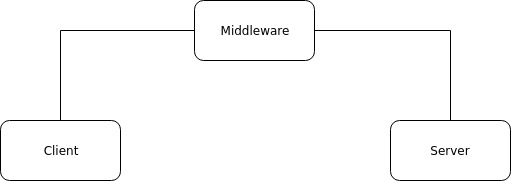
\includegraphics[scale=0.8]{../pictures/Komponenten.jpg}\\
\centerline{\textbf{Abbildung 1:} Komponentendiagramm}\\
\\Die Middleware soll dafür sorgen, dass ein entferntes Objekt wie ein lokales behandelt werden kann, ohne, dass der Anwender dies merkt. Dazu muss mit Hilfe eines Compilers und einer idl-Datei ein Stub-Objekt erzeugt werden.\\
Dieses Stub-Objekt kommuniziert über den Nameservice mit dem ObjectBroker des Servers, auf dem das richtige Objekt liegt. Die Antworten des Objektes werden direkt an ein RemoteObject, dass im Stub-Objekt die Kommunikation übernimmt, gesendet und vom Stub-Objekt in den richtigen Datentypen geparst, damit das Ergebnis direkt vom Client genutzt werden kann.\\
Der ObjectBroker vom Server, der im Nameservice hinterlegt ist, nimmt die Anfrage des Clients an und startet einen Dispatcher. Der Dispatcher leitet die Anfrage des Clients  an das passende LocalObject im MWareObjectWarehouse weiter, welches diese Anfrage parst und mittels Reflection im Objekt aufruft. Das Ergebnis dieses Aufrufs wird als String zurückgegeben und vom Dispatcher an den Client zurückgesendet.\\
\\
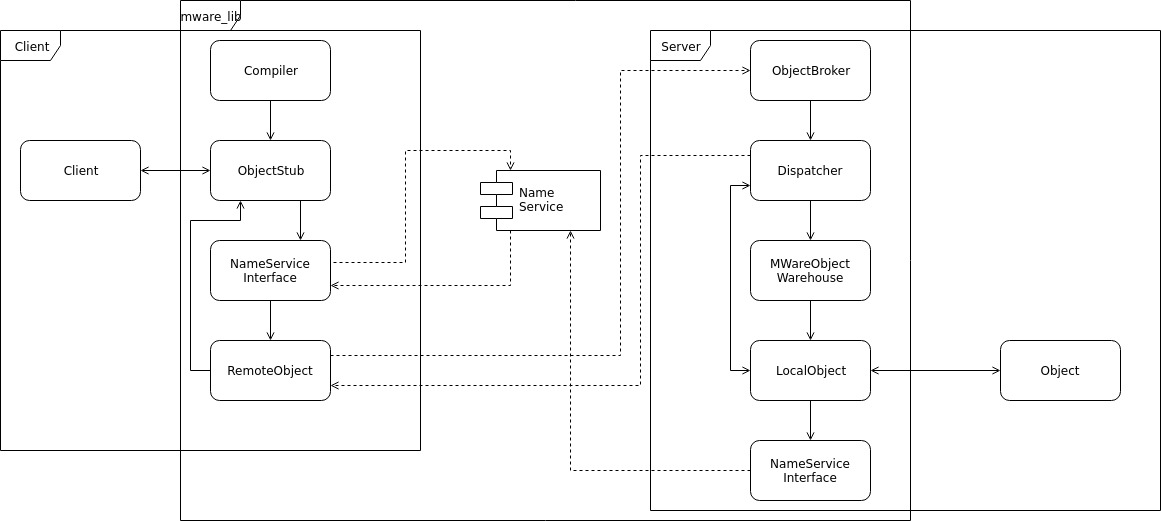
\includegraphics[scale=0.35]{../pictures/Baustein.jpg}\\
\centerline{\textbf{Abbildung 2:} Bausteindiagram Middleware}\\

\section{Protokoll}
Die Kommunikation der Middleware läuft über TCP-Sockets, daher muss ein eigenes Protokoll erstellt werden. Im folgenden wird das Protokoll beschreiben.

\subsection{Nameservice}
\subsubsection{Rebind}
Rebind bindet ein Objekt über die Hostadresse und den Port des Servers, auf dem das Objekt liegt, an den Nameservice
\begin{itemize}
\item \textbf{Aufruf:} rebind!<Name>:<Hostadresse>:<Port>
\item \textbf{Antwort:} ok
\end{itemize}

\subsubsection{Resolve}
Resolve fragt ein Objekt vom Nameservice ab. Zurückgegeben werden die Hostadresse und der Port des Servers, auf dem das angefragte Objekt liegt.
\begin{itemize}
\item \textbf{Aufruf:} resolve!<Name>
\item \textbf{Antwort:} ok:<Name>:<Hostadresse>:<Port>
\end{itemize}

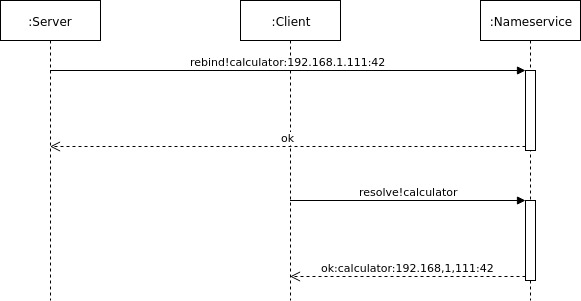
\includegraphics[scale=0.7]{../pictures/FlowChartNameService.jpg}\\
\centerline{\textbf{Abbildung 3:} Flowchart Nameservice}\\

\subsection{Middleware}
In der Middleware kommunizieren die RemoteObjekte mit den lokalen Objekten mit Hilfe des folgenden Protokolls:
\begin{itemize}
\item \textbf{Methodenaufruf:} <Objektname>!<Funktionsnname>![<Parameter>:<Datentyp>]*
\item \textbf{Antwort:} result:<Ergebnis>
\end{itemize}

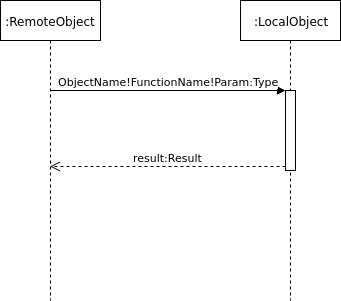
\includegraphics[scale=1]{../pictures/FlowChartObjectProtokol.jpg}\\
\centerline{\textbf{Abbildung 4:} Flowchart Objektkommunikation}\\

\subsection{Middleware}
\subsubsection{Aufruf einer Methode}
\begin{itemize}
\item \textbf{Aufruf:} resolve!<Name>
\item \textbf{Antwort:} ok:<Name>:<Hostadresse>:<Port>
\end{itemize}
 
\section{Nameservice}

Der Nameservice bildet ab, welches Objekt sich auf welchem Server befindet. Mit dem Namen des Objekts kann der Host und der Port des Servers, auf welchen das Objekt liegt, abgefragt und eine Verbindung dahin aufgebaut werden. Der Nameservice ist als entferntes Objekt zu implementieren, sodass die Nachrichtenübermittlung mittels TCP realisiert wird.

\subsection{Rebind}

\textbf{Beschreibung:}\\
Bindet ein Objekt mit dem übergebenen Namen im Nameservice.\\
Die zugehörigen Informationen sind Hostadresse und Port des Servers, auf dem das Objekt liegt. Bereits vorhandene Objekte mit dem selben Namen werden überschrieben.\\ \\
\textbf{Anfrage:} rebind!<Name>:<Hostadresse>:<Port>\\ \\
\textbf{Antwort:} ok\\ \\
\textbf{Beispiel:}
\begin{tabbing}
\textit{Server:}~~~~~~~~~~~ \= rebind!calculator:192.168.1.111:42 \\
\textit{Nameservice:} \> ok
\end{tabbing}
\textbf{Ablauf}
\begin{enumerate}
\item Auslesen von Name, Hostadresse und Port
\item Speichern der Hostadresse und des Ports unter angegebenen Namen
\item Rückgabe von ok
\end{enumerate}

\subsection{Resolve}

\textbf{Beschreibung:}\\
Fragt die zugehörigen Informationen zum Objekt mit dem übergebenen Namen ab.\\
Als Antwort werden Hostadresse und Port, die für den übergebenen Namen gespeichert wurden, zurückgegeben.\\ \\
\textbf{Anfrage:} resolve!<Name>\\ \\
\textbf{Antwort:} ok:<Name>:<Hostadresse>:<Port>\\ \\
\textbf{Beispiel:}
\begin{tabbing}
\textit{Client:}~~~~~~~~~~~ \=  resolve!calculator \\
\textit{Nameservice:} \> ok:calculator:192.168.1.111:42
\end{tabbing}
\textbf{Ablauf}
\begin{enumerate}
\item Auslesen vom Namen
\item Lesen der Hostadresse und des Ports unter angegebenen Namen
\item Rückgabe von ok:<Name>:<Hostadresse>:<Port>
\end{enumerate} 

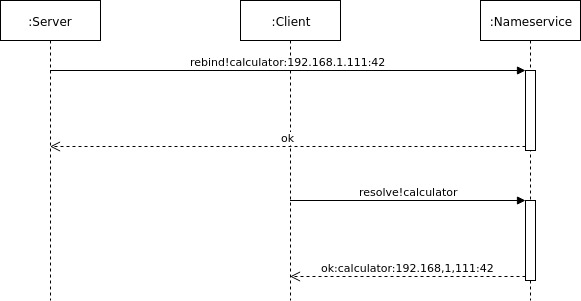
\includegraphics[scale=0.7]{../pictures/FlowChartNameService.jpg}\\
\centerline{\textbf{Abbildung 5:} Flowchart Nameservice}\\

\section{Middleware}
Aufgabe der Middleware ist es, den Zugriff auf entfernte Objekte so zu ermöglichen, dass die benutzenden Objekte nicht merken, dass es sich um ein entferntes Objekt handelt.\\
Im folgenden werde ich alle Module, die die Middleware beinhaltet, vorstellen.

\subsection{Object Broker}
Das "Frontend"  der Middleware.\\
Wird clientseitig von dem Stub-Objekt, das vom IDL-Compiler erzeugt wurde, angesprochen. Dieser clientseitige Object Broker sendet eine Anfrage mit dem Namen des Stub  Objektes an den Nameservice. Dieser liefert, sofern bekannt, die Hostadresse und den Port des Servers, auf dem das angefragte Objekt liegt, zurück.\\
Bekommt der anfragende ObjectBroker eine Hostadresse und einen Port zurück, stellt er dort eine Anfrage zur Ausführung der gewünschten Funktion. Der serverseitige Object Broker nimmt diese Anfrage entgegen und startet einen Dispatcher mit dem Socket des Clients.

\subsection{Dispatcher}
Der Dispatcher verarbeitet die Anfrage des Clients und ruft die angeforderte Methode des Objektes mit den übergebenen Parametern aus und leitet das Ergebnis oder auftretende Exceptions an den Client weiter. Danach wird die Verbindung geschlossen.

\subsubsection{Ablauf}
\begin{enumerate}
\item Empfangen der Nachricht vom Client
\item Auslesen des Namens vom Objektes, das angesprochen werden soll.
\item Anfrage an das Object Warehouse nach dem Objekt mit dem gegebenen Namen
\item Aufruf der angegebenen Methode
\item Rückgabe des Ergebnisses an den Client als Nachricht
\end{enumerate}

\subsection{Socket Controller}
Ist für die eigentliche Kommunikation verantwortlich. Sendet und empfängt Nachrichten über einen übergebenen Socket.

\subsubsection{Send Message}
\textbf{Beschreibung:}\\
Sendet eine Nachricht an das Objekt auf der "anderen Seite" des Sockets.\\ \\
\textbf{Aufruf:} sendMessage(String message)\\ \\
\textbf{Variablen}
\begin{enumerate}
\item \textbf{message:} Nachricht, die an den Kommunikationspartner gesendet werden soll
\end{enumerate}
\textbf{Ablauf}
\begin{enumerate}
\item Senden der übergebenen Nachricht an den Kommunikationspartner
\end{enumerate}

\subsubsection{Receive Message}
\textbf{Beschreibung:}\\
Empfängt eine Nachricht vom Kommunikationspartner.\\ \\
\textbf{Aufruf:} receiveMessage()\\ \\
\textbf{Ablauf}
\begin{enumerate}
\item Empfangen einer Nachricht an den Kommunikationspartner
\item Rückgabe der empfangenen Nachricht
\end{enumerate}

\subsection{Nameservice Interface}
Interface, dass den Nameservice anspricht.

\subsubsection{Rebind}
\textbf{Beschreibung:}\\
Spricht die Funktion Rebind des Nameservice an. Das Objekt wird mit Hilfe eines MWare-Objektes im Object Warehouse gespeichert und die IP-Adresse und der Port des Servers mit dem Namen des Objektes beim Nameservice registriert. \\ \\
\textbf{Aufruf:} rebind(Object servant, String name)\\ \\
\textbf{Variablen}
\begin{itemize}
\item \textbf{servant:} Objekt, dass beim Nameservice registriert wird
\item \textbf{name:} Name des Objektes, mit dem es beim Nameservice registriert wird
\end{itemize}
\textbf{Ablauf}
\begin{enumerate}
\item Erzeugen eines MWare-Objektes mit dem übergebenen Objekt
\item Einfügen des MWare-Objektes in das MWare Warehouse
\item Rebind-Anfrage an den Nameservice
\begin{itemize}
\item \textbf{Anfrage:} rebind!<Name>:<Hostadresse>:<Port>
\begin{itemize}
\item Name: Name des zu registrierenden Objektes 
\item Hostadresse: Eigene IP-Adresse, auf der der Server horcht
\item Port: Port, auf dem der Server horcht
\end{itemize}
\item \textbf{Antwort:} ok
\end{itemize}
\end{enumerate}

\subsubsection{Resolve}
\textbf{Beschreibung:}\\
Spricht die Funktion Resolve des Nameservice an. Die IP-Adresse und der Port des Servers, auf dem das Objekt mit dem übergebenen Namen liegt, wird zurückgegeben. \\ \\
\textbf{Aufruf:} resolve(String name)\\ \\
\textbf{Variablen}
\begin{itemize}
\item \textbf{name:} Name des Objektes, dass beim Nameservice abgefragt wird
\end{itemize}
\textbf{Rückgabe:} Objektreferenz des angefragten (entfernten) Objektes\\ \\
\textbf{Ablauf}
\begin{enumerate}
\item Erzeugen eines MWare-Objektes mit dem übergebenen Objekt
\item Einfügen des MWare-Objektes in das MWare Warehouse
\item Rebind-Anfrage an den Nameservice
\begin{itemize}
\item \textbf{Anfrage:} rebind!<Name>:<Hostadresse>:<Port>
\begin{itemize}
\item Name: Name des zu registrierenden Objektes 
\item Hostadresse: Eigene IP-Adresse, auf der der Server horcht
\item Port: Port, auf dem der Server horcht
\end{itemize}
\item \textbf{Antwort:} ok
\end{itemize}
\end{enumerate}

\subsection{Object Warehouse}
Verwaltet sowohl lokale aus auch entfernte Objekte für den Zugriff.

\subsubsection{Add Object}
\textbf{Beschreibung:}\\
Fügt ein Objekt zum Warehouse hinzu. \\ \\
\textbf{Aufruf:} addObject(String name, MWareObject object)\\ \\
\textbf{Variablen}
\begin{itemize}
\item \textbf{name:} Name des Objektes, dass hinzugefügt werden soll
\item \textbf{object:} Objektes, dass hinzugefügt werden soll
\end{itemize}
\textbf{Rückgabe:} Boolean, ob das Objekt hinzugefügt wurde, oder nicht.\\ \\
\textbf{Ablauf}
\begin{enumerate}
\item Prüfen, ob bereits ein Objekt mit dem Namen vorhanden ist
\begin{itemize}
\item Wenn ja: Rückgabe von false
\item Wenn nein: Hinzufügen des Objekts unter angegebenen Namen und Rückgabe von true
\end{itemize}
\end{enumerate}

\subsubsection{Remove Object}
\textbf{Beschreibung:}\\
Entfernt ein Objekt vom Warehouse. \\ \\
\textbf{Aufruf:} removeObject(String name)\\ \\
\textbf{Variablen}
\begin{itemize}
\item \textbf{name:} Name des Objektes, dass entfernt werden soll
\end{itemize}
\textbf{Rückgabe:} Boolean, ob das Objekt entfernt wurde, oder nicht.\\ \\
\textbf{Ablauf}
\begin{enumerate}
\item Prüfen, ob ein Objekt mit dem Namen vorhanden ist
\begin{itemize}
\item Wenn ja: Entfernen des Objektes und Rückgabe von true
\item Wenn nein: Rückgabe von false
\end{itemize}
\end{enumerate}

\subsubsection{Replace Object}
\textbf{Beschreibung:}\\
Fügt ein Objekt zum Warehouse hinzu. \\ \\
\textbf{Aufruf:} replaceObject(String name, MWareObject object)\\ \\
\textbf{Variablen}
\begin{itemize}
\item \textbf{name:} Name des Objektes, dass hinzugefügt werden soll
\item \textbf{object:} Objektes, dass hinzugefügt werden soll
\end{itemize}
\textbf{Ablauf}
\begin{enumerate}
\item Prüfen, ob bereits ein Objekt mit dem Namen vorhanden ist
\begin{itemize}
\item Wenn ja: Ersetzen des vorhandenen Objektes mit dem übergebenen
\item Wenn nein: Hinzufügen des Objekts unter angegebenen Namen
\end{itemize}
\end{enumerate}

\subsubsection{Get Object}
\textbf{Beschreibung:}\\
Liefert das Objekt mit dem übergebenen Namen zurück, sofern vorhanden. \\ \\
\textbf{Aufruf:} getObject(String name)\\ \\
\textbf{Variablen}
\begin{itemize}
\item \textbf{name:} Name des Objektes, dass hinzugefügt werden soll
\end{itemize}
\textbf{Rückgabe:} Objekt mit dem übergebenen Namen, wenn vorhanden.\\ \\
\textbf{Ablauf}
\begin{enumerate}
\item Prüfen, ob bereits ein Objekt mit dem Namen vorhanden ist
\begin{itemize}
\item Wenn ja: Rückgabe des Objekts
\item Wenn nein: Rückgabe von null
\end{itemize}
\end{enumerate}

\subsection{MWareObject}
Kann sowohl ein lokales, als auch ein entferntes Objekt repräsentieren und ruft die Methoden des Objektes auf.

\subsubsection{Call Method}
\textbf{Beschreibung:}\\
Ruft die in der übergebenen Nachricht angegebene Methode mit den angegebenen Parametern auf. \\ \\
\textbf{Aufruf:} callMethod(String message)\\ \\
\textbf{Variablen}
\begin{itemize}
\item \textbf{message:} String mit allen Informationen zur aufgerufenen Methode
\begin{itemize}
\item \textbf{Format:} <Name>!<Methode>![Parameter:Datentyp]*
\end{itemize}
\end{itemize}
\textbf{Rückgabe:} Ergebnis des Methodenaufrufs als String.\\ 
\textbf{Format:} result:<Ergebnis>.\\ \\
\textbf{Ablauf}
\begin{enumerate}
\item Parsen des übergebenen Strings mittels des oben angegebenen Formats
\item Aufruf der angegebenen Funktion mit den übergebenen Parametern
\item Rückgabe des Ergebnisses im Format: result:<Ergebnis>
\end{enumerate}

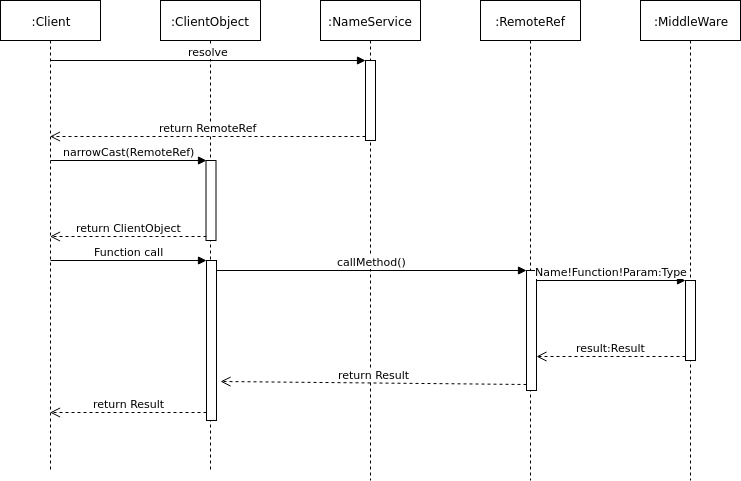
\includegraphics[scale=0.6]{../pictures/ClientFlowChart.jpg}\\
\centerline{\textbf{Abbildung 4:} Flowchart Client}\\

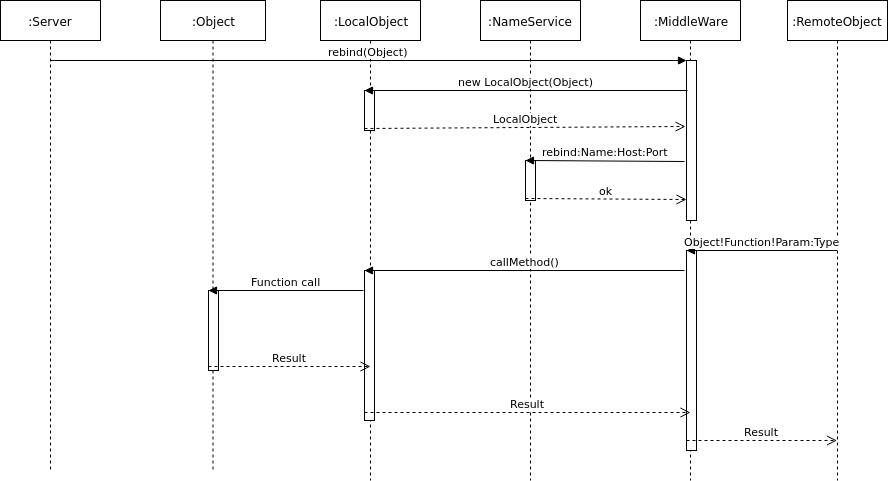
\includegraphics[scale=0.5]{../pictures/ServerFlowChart.jpg}\\
\centerline{\textbf{Abbildung 4:} Flowchart Server}

\section{IDL-Compiler}
Der IDL-Compiler muss die IDL-Datei einlesen und daraus zwei Java-Dateien erzeugen.
\begin{enumerate}
\item \_ClassNameImplBase.java - Abstrakte Klasse, die die Methoden der Klassen aus der IDL-Datei als abstrakte Methoden beinhaltet
\begin{enumerate}
\item Muss Methode narrowCast beinhalten, die ein Objekt zurückliefert, welches mittels des Objektes aus dem Resolve-Aufruf das RemoteObject ansprechen kann
\end{enumerate}
\item ClassName.java - Klasse, die die jeweiligen Methoden des entfernten Objektes aufruft.
\end{enumerate}
Die IDL-Datei ist folgendermaßen aufgebaut:
\begin{lstlisting}
module modulename {    // Name des Moduls
	class ClassA {    // Name der Klasse
		string methodA(int a);    // Methode der Klasse
	};    // Klassenende
	class ClassB {    // Zweite Klasse
		double methodA(double param1, double param2);
		int methodB(int param1);
	};
};    // Modulende
\end{lstlisting}

Das Modul beschreibt ein Java-Package, dass mehrere Klassen beinhalten kann. Dies muss mittels \\
package modulename;\\
in den Java-Klassen vermerkt werden.

\subsection{Abstrakte Klasse}

\subsubsection{narrowCast}
\textbf{Beschreibung:}\\
Liefert ein Objekt zurück, dass ein Objekt der erzeugten Klasse zurückliefert.\\ \\
\textbf{Aufruf:} sendMessage(Object rawObjectReference)\\ \\
\textbf{Variablen}
\begin{enumerate}
\item \textbf{rawObjectReference:} Objekt, dass vom Nameservice zurückgeliefert wird (MWareObject)
\end{enumerate}

\subsection{Ausführbare Klasse}
Die ausführbare Klasse muss alle Funktionen inklusive der Implementierung des Methodenaufrufs beinhalten. Siehe hierfür das Kapitel 2.3.6 CallMethod.
% first example chapter
% @author Thomas Lehmann
%
\chapter{Lösungsweg}

\section{Nameservice}
Der Nameservice durfte gemäß den Vorgaben nicht in Java implementiert werden, daher entschied ich mich für Python.
Abgebildet werden die Objekte in einem Dictionary, in dem Key-Value-Paare gespeichert werden können.\\
Der Schlüssel für das jeweilige Objekt ist der Name des Objektes und der Wert dazu ist wieder ein Dictionary. Dieses Dictionary hat zwei Keys, zum einen mit dem Key "host", die als Wert die IP-Adresse des Servers, auf dem das Objekt liegt, hat und den Key "port", der als Wert die Portnummer hat.\\
\\Geht eine Anfrage beim Nameserver an, wird ein Thread gestartet, in dem die eingehende Nachricht ausgewertet wird. Die jeweilige gewünschte Funktion (resolve oder rebind) wird ausgeführt und das Ergebnis zurückgegeben.\\
Wird ein Objekt beim Nameservice gebunden, werden Hostadresse und Portnummer mittels Protokoll übertragen. Diese beim Namesservice eingegangene Nachricht wird dann über eine Split-Funktion aufgeteilt und die Adresse und der Port zum übergebenen Namen hinterlegt.\\
Wird ein Objekt beim Nameservice angefragt, werden sofern vorhanden die IP-Adresse und der Port mittels des dafür angefertigten Protokolls zurückgegeben. Ist es nicht vorhanden, wird "nok:Unknown Object" zurückgegeben.\\

\subsection{Ablauf innerhalb des Nameservice}
\begin{itemize}
\item Entgegennahme der Anfrage
\item Starten eines Threads mit dem Socket
\item Empfangen der Nachricht
\item Aufteilen der Nachricht mittels Split-Funktion beim Ausrufezeichen 
\item Auswerten des ersten Teils der Nachricht (Aufgerufene Funktion)
\begin{enumerate}
\item rebind - Weitergabe des zweiten Nachrichtenteils an die Funktion rebind - Ergebnis = Rückgabewert
\item resolve - Weitergabe des zweiten Nachrichtenteils an die Funktion resolve - Ergebnis = Rückgabewert
\item Sonstiges - Ergebnis = "nok:unknown message"
\end{enumerate}
\item Senden des Ergebnisses über den Socket
\item Schließen des Sockets
\end{itemize}

\subsection{Ablauf rebind}
\begin{itemize}
\item Aufsplitten des zweiten Nachrictenteils mittels Splitfunktion am Doppelpunkt
\item Erstellen eines Dictionarys, das Host-Adresse und Port beinhaltet
\item EIntragen des Dictionary in das des Nameservice mit dem Namen als Key
\item Rückgabe von "ok"
\end{itemize}

\subsection{Ablauf resolve}
\begin{itemize}
\item Abfrage des Objektes mit dem übergebenen Namen
\begin{enumerate}
\item Wenn vorhanden, zusammenbau des Rückgabestrings: "ok:<Name>:<Hostadresse>:<Port>"
\item Wenn nicht vorhanden: Rückgabestring = 	"nok:no object"
\end{enumerate}
\item Rückgabe des Rückgabestrings
\end{itemize}

\section{Middleware}

\subsection{Object Broker}
Der ObjectBroker ist das FrontEnd der Middleware. Hier kann die Referenz zum Nameservice amgefragt werden. In meiner Implementierung kann auch direkt ein Objekt über den ObjectBroker mittels Funktion addObject(Object object) hinzugefügt werden. Diese ruft allerdings auch nur die Funktion rebind des Nameservice auf.\\
Wird ein ObjectBroker erzeugt, wird automatisch ein Thread gestartet, der auf einem zufällig gewählten Port horcht. Gehen Anfragen ein, wird ein Dispatcher gestartet, der Anfragen entgegen nimmt und die Funktionen der lokalen Objekte mittels Reflection aufruft.

\subsubsection{Ablauf ObjectBroker}
\begin{itemize}
\item Starten eines ServerSockets
\item Horchen auf dem Port (hier ein zufällig erstellter)
\item Bei eingehenden Anfragen: Erstellen eines neuen Dispatchers und starten des Dispatcher-Threads mittels start()
\end{itemize}

\subsubsection{Ablauf Dispatcher}
\begin{itemize}
\item Empfangen der Nachricht
\item Splitten der Nachricht, um den Namen des angefragten Objektes zu bekommen
\item Abfrage des Objektes im ObjectWarehouse
\item Aufruf der Funktion callMethod(message) mit der empfangenden Nachricht als Parameter
\item Rückgabe des Ergebnisses von callMethod 
\end{itemize}

\subsection{ObjectWarehouse}
Das ObjectWarehouse speichert alle MWareObjekte, damit sowohl lokale als auch entfernte Objekte über die MiddleWare verwendet werden können. Zwar sollten keine lokalen Objekte über die MiddleWare benutzt werden, aber so wird unnötige Netzauslastung verhindert, falls doch ein lokales Objekt angesprochen werden soll.\\
Das ObjectWarehouse kann vom ObjectBroker, vom Dispatcher und vom Nameservice angesprochen werden.

\subsection{MWareObject}
Das MWareObject ist ein Interface, dass von den Klassen LocalObject und RemoteObject implementiert wird. Es schreibt folgende Methoden vor:
\begin{enumerate}
\item String getName(); - Liefert den Namen des Objekts zurück
\item String callMethod(String message); - Führt die Funktion aus, die laut der übergebenen Nachricht aufgerufen werden soll
\end{enumerate}

\subsection{LocalObject}
Die Klasse LocalObject ist ein Wrapper für alle Objekte, die im Nameservice gebunden werden. Hier wird mittels Funktion callMethod die aufzurufende Funktion mit Hilfe von Reflection ausgeführt

\subsubsection{Ablauf callMethod}
\begin{enumerate}
\item Aufsplitten der Nachricht, um Methodennamen, Parameter und ihre Datentypen zu extrahieren
\item Suchen der Funktion durch Name und Class-Array mit Datentypen der Parameter
\item Aufruf der Funktion mittels Funktion invoke, Parameter: Referenz des Objekts und Object-Array mit Datentypen
\item Rückgabe des Ergebnisses aus dem Funktionsaufruf als String mit "result:" als Präfix
\item Treten beim Aufruf Exceptions auf, werden diese gefangen und der Aufrufer wird darüber mittels der Antwort "exception:<ExceptionClass>:<ExceptionMessage>" darüber benachrichtigt 
\end{enumerate}

\subsection{RemoteObject}
Das RemoteObject ist der Kommunikationspartner des Dispatchers und wird vom NameServiceInterface zurückgeliefert. Es speichert die Hostadresse und den Port des Servers, auf dem das LocalObject liegt. Wird die Funktion callMethod aufgerufen, wird ein Socket erstellt und der Dispatcher dazu angeleitet, die Funktion des lokalen Objekts aufzurufen. Das Ergebnis wird direkt zurückgeliefert.

\subsubsection{Ablauf callMethod}
\begin{itemize}
\item Erstellen eines Sockets mit der gespeicherten Hostadresse und dem Port
\item Senden der Nachricht über den Socket
\item Empfangen der Antwort
\item Rückgabe der Antwort
\end{itemize}

\section{IDL-Compiler}
Der IDL Compiler wandelt IDL-Dateien in die in der Datei beschriebenen Klassen um. Aus jeder beschriebenen Klasse wird jeweils eine Abstrakte Klasse und eine Klasse mit Implementierung erzeugt.

\subsection{Ablauf}
\begin{itemize}
\item Einlesen der Datei
\item Speichern des Modulnamens
\item Einlesen der Klassen und ihrer Funktionen mit Parametern
\item Speichern der Klassen, Funktionen und Parametern als Objekte
\item Umwandeln der Klassen mit ihren Funktionen und deren Parametern in die Abstrakten Klassen
\item Schreiben der Funktion narrowCast, bei der ein Objekt aus dem NameService übergeben werden kann
\begin{enumerate}
\item Das übergebene Objekt wird zu einem MWareObject gecastet und damit wird ein neues Objekt der Klasse mit Implementierung erzeugt und zurückgegeben
\end{enumerate}
\item Erzeugen der Klasse mit Implementierung, bei der die jeweilige Funktion mit ihren Parametern als String zusammengebaut wird, dass mit diesem die Funktion callMethod des MWareObjects aufgerufen werden kann.
\begin{enumerate}
\item Aufruf der Funktion mit dem zusammengebauten String
\item Casten der Antwort auf den Rückgabetypen der Funktion und Rückgabe des Ergebnisses
\end{enumerate}
\end{itemize}
% first example chapter
% @author Thomas Lehmann
%
\chapter{Fazit}
Nach anfänglicher Planlosigkeit bei dieser Aufgabe, machte ich mir genauere Gedanken, wie ich diese angehen könnte und las mir noch einmal die Folien der Aufgabenvorstellung durch. Desto mehr ich mich damit beschäftigte, desto mehr Ideen kamen mir zur Implementierung. Ich entschied mich, diesen Lösungsansatz zu implementieren. \\
Danach ging der Entwurf erst relativ leicht von der Hand. Nachdem ich jedoch mit der Implementierung begann, musste ich den Entwurf einige male abändern, da meine Ideen so nicht ganz funktionierten.\\
Vor allem aber das Testen bereitete mir Probleme. Da die einzelnen Module relativ schwierig zu testen sind, musste ich erst alle Module fertigstellen, um vernünftig testen zu können. Zwar hätte man für jedes Modul  ein ausgiebiges Teststsystem schreiben kännen, jedoch hätte dies meinen zeitlichen Rahmen gesprengt. \\
Dadurch, dass ein vernünftiges Testen erst möglich war, wart es auch schwierig, auftretende Fehler zu entdecken. Dies gelang jedoch dank der Debug-Ausgaben sehr gut. \\ 
Das gegebene Testszstem bereitete noch einmal Probleme, da mein System zwar mit meinen Tests funktionierte, hier jedoch anfänglich neue Fehler auftraten. Diese Fehler traten auf, weil z.B. mein Nameservice in einem Subpackage lag und falsch benannt war. Hier wurde als Fehler angezeigt, dass  die Funktion getNameservice nicht vorhanden sei. Diese war aber implementiert. Ein Versuch, den Nameservice umzubenennen und in das Hauptpackage zu verschieben war jedoch erfolgreich.\\
Ein zweiter Fehler trat auf, da ich die Funktion shutDown nicht implementiert hatte. Diese konnte jedoch leicht nachimplementiert werden.\\
Der Compiler war ebenfalls eine Herausforderung. Hierbei orientierte ich mich an dem Compiler, der von Herrn Schulz bereitgestellt wurde. Ich entschied mich jedoch, nicht mit statischen Variablen zu arbeiten, da dies in meinen Augen keinen Sinn machte, da die Zeichen ziemlich kurz sind und ich so schneller implementieren konnte. Eine Änderung des Compilers war ja sowieso nicht vorgesehen.

%\bibliographystyle{plain}
%\bibliographystyle{dinat}
%\bibliography{literature}

% Appendix
%\appendix
%% !TEX root = ../thesis.tex
% appendix example chapter
% @author Thomas Lehmann
%

\chapter{Anhang}
\lipsum


%\IGlossary

\Istatement

\end{document}
